\chapter{VQE for physical models}
\label{chap:vqe_numerics}

In this chapter we start investigating the algorithm called variational quantum eigensolver (VQE), which is arguably the flagship algorithm of the VQA family. We will give an overview of the known physical an numerical experiments, as well as present our own results in investigating the properties of VQE solutions.



\section{Ansatz dependence and depth scaling}

In this section, we will summarize what is known about the performance of VQE on a number of model problems. Typically, these problems are lattice problems because it is easy to study scaling with the number of qubits $n$ by just increasing the lattice. For molecular Hamiltonians, the only easy way to scale the problem up is to increase the size of the active space. Even changing the basis of orbitals leads to a different family of problems, strictly speaking.

A number of papers studied how the error of VQE behaves as a function of ansatz depth for different models. Quite often, the error was found to decrease exponentially with the depth of the ansatz. This was observed for the Hubbard model by Cade et al.~\cite{cade_strategies_2019} and also observed by us for the Hubbard model with the next-nearest neighbor Coulomb interactions \cite{uvarov_variational_2020}. Later, the same behavior was also observed for the Heisenberg model on the kagome lattice \cite{kattemolle_variational_2021,bosse_probing_2021}. 

On the other hand, some problems exhibit a threshold in the optimization error with increasing depth. For example, Ref.~\cite{bravo-prieto_scaling_2020} studies transverse field Ising and Heisenberg models for a 1D chain with open boundary conditions and finds two regimes in the behavior. Before the threshold depth, the error decays polynomially in depth, whereas after the threshold the convergence is exponential. The location of the threshold itself also moves with the number of qubits, seemingly linear with $n$. This threshold appears not only in the hardware efficient ansatz, like in Ref.~\cite{bravo-prieto_scaling_2020}, but also in the Hamiltonian variational ansatz as well \cite{wiersema_exploring_2020}. A similar threshold behavior was also observed in optimizing the ansatz to get to a target unitary \cite{kiani_learning_2020,campos_abrupt_2020}.

Recent findings connect this kind of threshold behavior to the dimensionality of the Lie algebra associated with the ansatz circuit \cite{larocca_theory_2021}. When the effective dimension\footnote{The ansatz can be treated as a differentiable function from $\mathbb
{R}^k \rightarrow \mathbb{C}^{2^n}$. One way to define effective dimension is to take the maximum rank of its Jacobian. Alternatively, the dimension is defined in terms of the Fisher information matrix, however that is essentially the same.} of the ansatz exceeds said dimension, the ansatz is said to be overparametrized. Apparently, in the overparametrized regime, the optimization landscape loses all the suboptimial minima, although the good behavior of the landscape may very well happen before the overparametrization. 
% We further investigate the ideas related to the effective dimension of the ansatz in Chapter \ref{chap:dla}.



\section{VQE for spin models}

\subsection{Transverse field Ising model}

The first simple example of an interesting system for VQE testing is the transverse field Ising (TFI) model with periodical boundary conditions:

\begin{equation}\label{eq:tfim}
    H_\mathrm{TFIM}=J\sum\limits_{i=1}^n Z_i Z_{i+1} + h\sum\limits_{i=1}^n X_i, \; J>0, \; h>0.
\end{equation}

This model has trivial product state solutions for $h = 0$ and for $J = 0$, but for other values of the parameters the solution is an entangled state. The model is still integrable: the Jordan--Wigner transformation maps it to a system of free fermions \cite{lieb_two_1961}. This fact makes it possible to use the TFI model to test VQE and its variants even outside numerical simulations. 

\begin{figure}
    \centering
    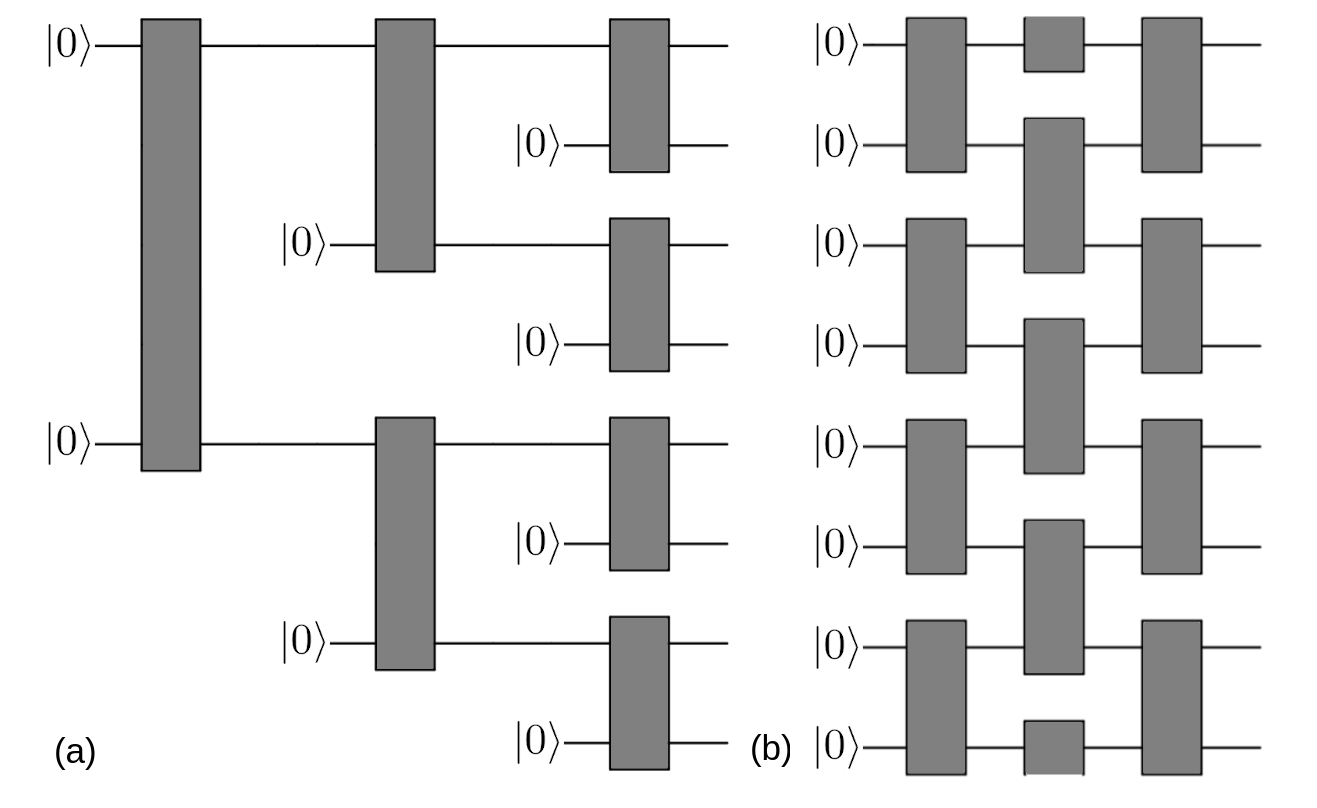
\includegraphics[width=0.7\textwidth]{figures/tree_and_checkerboard_circuit.png}
    \caption{(a) Tree tensor network state. (b) Checkerboard tensor
    network state. In both cases, the quantum register is instantiated in
    the $\ket{0}^{\otimes n}$ state and subject to entangling gates. Black boxes indicate
    two-qubit gates specified by Fig. \ref{fig:entangler}. Each block is
    parametrized independently. Reprinted from \cite{uvarov_machine_2020}}.
    \label{fig:tree_and_checkerboard}
\end{figure}

We studied this model numerically for 10 qubits. We tested VQE solutions for a variety of different ansatz circuits:

\begin{enumerate}
    \item The \textit{rank-1 ansatz} simply consists of $R_Y$ and $R_Z$ gates applied to each qubit. The name stems from the fact that the state does not generate any entanglement: whatever qubit partition one selects, the Schmidt rank of the bipartition will always be equal to one.
    \item The \textit{tree tensor network ansatz} is depicted in Figure \ref{fig:tree_and_checkerboard}a. This ansatz provides entanglement between even the farthest of qubits, but the entanglement across any bipartition does not exceed $O(1)$ ebits: any contiguous region can be isolated by $O(1)$ cuts. It is possible to contract $\bra{\psi_{tree}} A \ket{\psi_{tree}}$ classically with $A$ being a local observable and $\ket{\psi_{tree}}$ being a tree tensor network state. 
    \item The \textit{checkerboard ansatz} consists of two-qubit blocks arranged in a checkerboard pattern Figure \ref{fig:tree_and_checkerboard}b. This ansatz can be expanded to obtain arbitrary precision, at the cost of having more parameters to optimize.
\end{enumerate}

Figure \ref{fig:tree_and_checkerboard} depicts the last two ans\"atze are with placeholder blocks. That is because they merely outline the structure of the circuit, while the content of these blocks may be more or less arbitrary. There is some tradeoff in this regard: if the blocks have more controllable parameters, they typically enable a richer set of states, but they as well become harder to optimize. Conversely, simpler blocks lead to poorer ansatz circuits which might be easier to optimize. In this experiment, we used a moderate-sized two-body ansatz that mostly uses the operators from the problem at hand, see Figure \ref{fig:entangler}. The unitary prepared by this block is described by the following equation:
\begin{equation}
    \label{eq:two_qubit_block1}
    U(\boldsymbol{\tilde{\theta}}) = (R_z(\tilde{\theta}_5) \otimes R_z(\tilde{\theta}_4)) \
    \circ R_{zz}(\tilde{\theta}_3) \ \circ  \ (R_x(\tilde{\theta}_1) \otimes R_x(\tilde{\theta}_2)),
\end{equation}
where $R_z (\theta) = e^{i\theta Z/2}$, $\ R_x (\theta) = e^{i\theta X/2}$, and $R_{zz} (\theta) = e^{i\theta Z\otimes Z/2}$. Thus, a complete ansatz would have five free parameters per two-qubit block.

\begin{figure}
    \centering
    \mbox{
    \Qcircuit @C=1.0em @R=1.0em {
           & \gate{e^{-i \tilde{\theta}_1 X}} & \multigate{1}{e^{-i \tilde{\theta}_3 {Z} \otimes {Z}}} & \gate{e^{-i \tilde{\theta}_4 Z}} & \qw \\
           & \gate{e^{-i \tilde{\theta}_2 X}} & \ghost{e^{-i \tilde{\theta}_3 Z \otimes Z}} & \gate{e^{-i \tilde{\theta}_5 Z}} & \qw \\
       }
    }
    \caption{Two-qubit entangler gate used in preparation of the states. The circuit is to be read left to right.}
    \label{fig:entangler}
\end{figure}

In our numerical implementation, we use Qiskit \cite{aleksandrowicz_qiskit:_2019} to simulate quantum circuits and the limited Broyden–Fletcher–Goldfarb–Shanno method (L-BFGS-B) to update the parameters during the classical step of VQE. We scan values of $h$ from $0$ to $2J$. For $h=0$, the optimization process started from a random point, then each additional point begins from the previous solution. This procedure is also known as AAVQE \cite{garcia-saez_addressing_2018}, except that, unlike AAVQE, we are also interested in all the intermediate points of the trajectory. To eliminate any obviously sub-optimal solutions, we also ran the scanning in the opposite direction, and for each value of the field we kept the better result.

The results are plotted in Figure \ref{fig:dE_ising}. All ans\"atze demonstrate an increase in the error in the vicinity of the phase transition point. Interestingly enough, tree tensor network ansatz does not yield any improvement against the rank-1 ansatz, nor does one layer of the checkerboard ansatz. As should be expected, increasing the depth of the checkerboard ansatz substantially improves the energy error of the solution. At $h = 0$, the ground state is degenerate. At nonzero values of the field, this degeneracy is lifted, but the spectral gap is very small. Nonetheless, the overlap of VQE solution in this regime is never smaller than $1/2$, and gradually moves to $1$ across the phase transition. At $h = 1.2$, the point where the energy error is the worst, the overlap of the VQE solution with the ground state is equal to 0.92. Just as observed in more detail for the Hubbard model in Section \ref{sec:hubbard}, the convergence in energy looks exponential in the depth of the circuit: the peaks of the curves are nearly halved with each new layer. 

What is unexpected is that the location of the peak is different for each depth. The offset of the peaks alone could be attributed to the finite-size effect, but this dependendce on the depth suggests that the entanglement structure is different across the range of $h$.

\begin{figure}
    \centering
    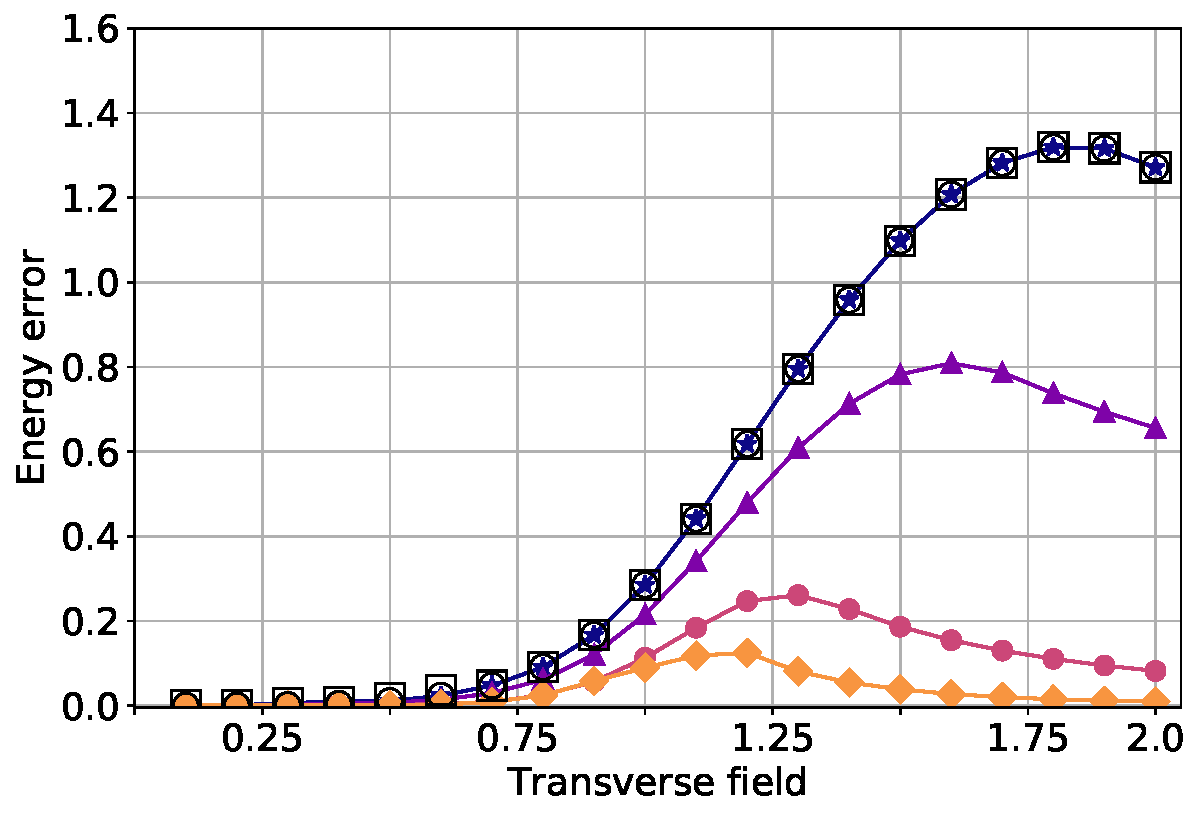
\includegraphics[width=0.7\textwidth]{figures/dE_ising.pdf}
    \caption{Absolute value of the difference in energy between the exact solution and VQE solutions for the transverse field Ising model. Hollow squares: rank-1 ansatz, hollow circles: tree tensor network, filled markers: checkerboard states ($\bigstar$: 1 layer, $\blacktriangle$: 2 layers, $\bullet$: 3 layers, $\blacklozenge$: 4 layers). Reprinted from \cite{uvarov_machine_2020}.}
    \label{fig:dE_ising}
\end{figure}

\subsection{Transverse-field Heisenberg model}

\begin{figure}
    \centering
    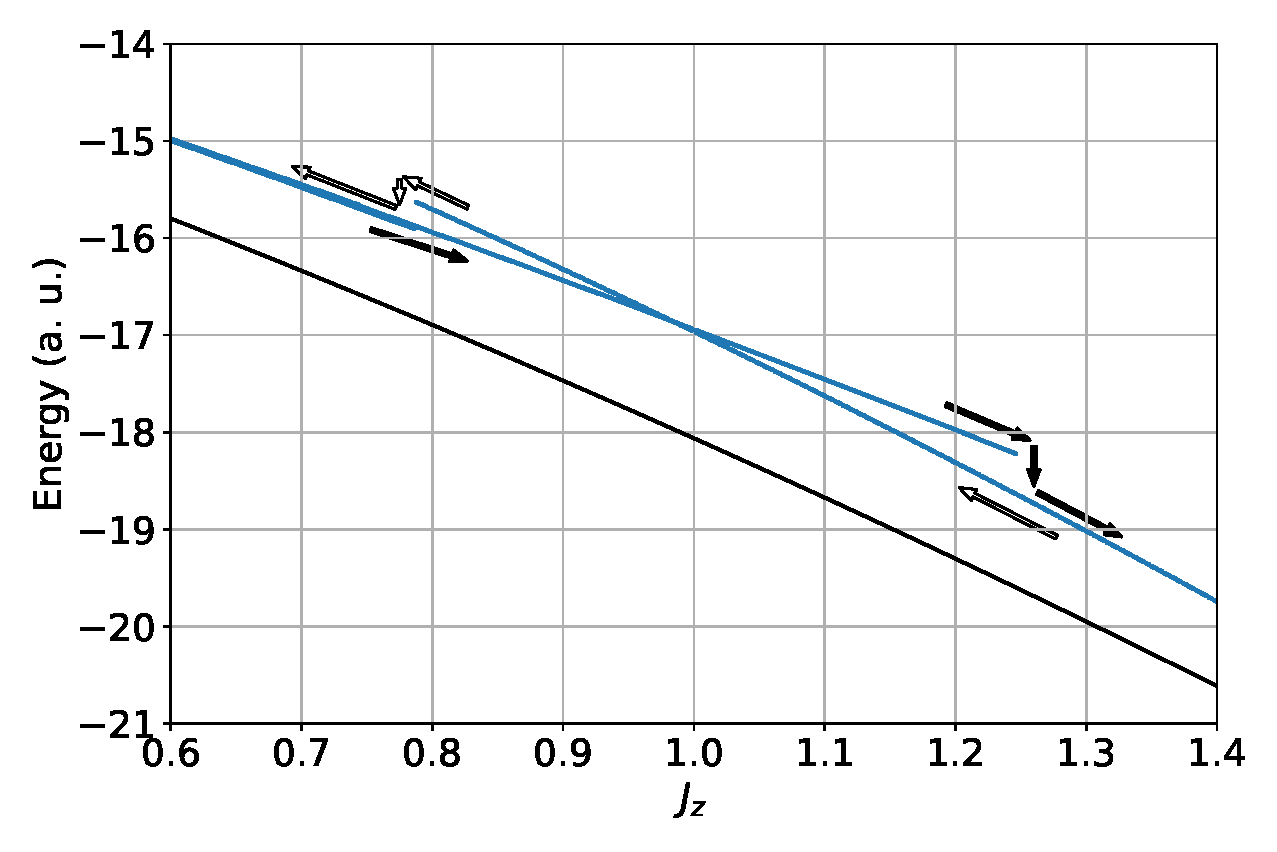
\includegraphics[width=0.7\textwidth]{figures/vqe_hysteresis_xxz_new.eps}
    \caption{Ground-state energy estimate for the XXZ model found
    in VQE sweeps. Filled (empty) arrows guide the eye along the
    “up” (“down”) sweep. The best solution out of two sweeps was
    subsequently used to train the classifier. The black line denotes the energy of the exact solution. Reprinted from \cite{uvarov_machine_2020}.}
    \label{fig:vqe_hysteresis}
\end{figure}

\begin{figure}
    \centering
    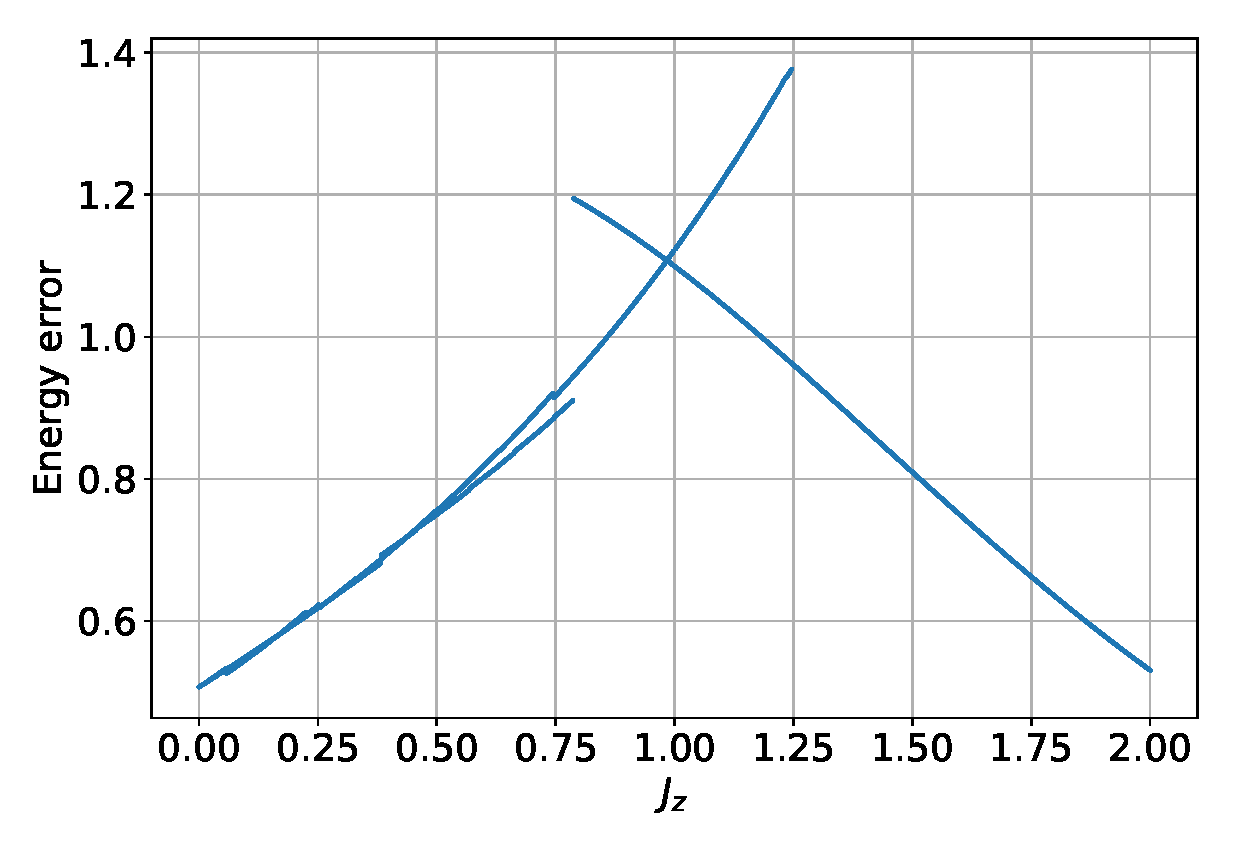
\includegraphics[width=0.7\textwidth]{figures/dE_xxz_best.eps}
    \caption{Energy difference between the exact solution and the ansatz solutions for the XXZ model.}
    \label{fig:dE_xxz}
\end{figure}

The XXZ Heisenberg model is defined as follows:

\begin{equation}
    \label{eq:heisenberg_xxz}
    H = \sum_{i=1}^n \left[J_\perp\left(X_i X_{i+1} + Y_i Y_{i+1}\right)
        + J_z Z_i Z_{i+1}\right].
\end{equation}

This model exhibits a more complicated behavior than the TFI model. However, for now we will only note that it, too, has a phase transition at $J_z = 1$. In Chapter \ref{chap:qml}, we study this model alongside the TFI model in context of quantum machine learning. Here we show the results of the same numerical experiments as for the TFI model, except that we only use the best ansatz (checkerboard with 4 layers).

In the experiments with the XXZ model, we observed an interesting peculiarity in the behavior of AAVQE. We found that the direction of the AAVQE sweep matters a lot. In the setup of AAVQE discussed in the original paper \cite{garcia-saez_addressing_2018}, the Hamiltonian is an easy one at the start and a difficult one at the finish. For models like ours, the behavior of the Hamiltonian along the change of $J_z$ is ``easy-hard-easy''. As such, to understand the low-energy properties of the model at different values of $J_z$, we could in principle run AAVQE in either direction. 

Figs.~\ref{fig:vqe_hysteresis}, \ref{fig:dE_xxz} show the results of running AAVQE in different directions. It turns out that the solutions in this case are susceptible to a hysteresis behavior: for a while after crossing the phase transition point, the solver stays in a suboptimal solution. Afterwards, the solution is suddenly changed to the optimal. Surprisingly enough, that behavior was not observed for the TFI model.

\section{VQE for Hubbard-like models}
\label{sec:hubbard}

\subsection{Next-nearest neighbor Hubbard model}

In condensed matter physics, frustrated systems with inhomogeneous interactions are hard to analyze owing to extra degrees of freedom to show up. On the one hand, strong electron-electron interactions precludes perturbative expansion over single-electron wave functions. On the other hand, more advanced numerical approaches to strongly correlated systems, e.g.~based on dynamical mean-field theory, treat the systems on a purely local manner. Whether modern quantum algorithms can give an edge in analyzing these models is an intensely studied question \cite{cade_strategies_2019,rungger_dynamical_2019,jaderberg_minimum_2020}. In this section, we analyze the performance of VQE for a one-dimensional model of spinless electrons with nearest- and next-nearest-neighbor interactions. This model represents a simple theoretical testbed to explore the physical properties of frustrated systems. Resulting from the competition between two types of interactions, a metallic state emerges even for strongly interacting systems. Interestingly, results of numerical simulations for finite size clusters unambiguously reveal that the ground state does not belong to the Luttinger liquid universality class \cite{Zhuravlev1997,zhuravlev_breakdown_2000,zhuravlev_one-dimensional_2001,Hohenadler2012,Karrasch2012}.

The frustrated systems are typically modeled using different variations of the Hubbard model. Physically, the model represents a lattice of atomic sites. Each site can have one or more energy levels for each spin. Electrons can hop between identical levels in different sites. The complicated part of the model is the Coulomb repulsion between the electrons sharing the same site or residing in neighboring sites. For simplicity, we consider the sites that have only one energy level to occupy. The Hamiltonian for such a model is as follows:

\begin{equation}
    H_{\text{Hubbard}} = \sum_{i \in [n], \sigma \in \{\uparrow, \downarrow\}} \epsilon_{i \sigma} \hat{n}_{i \sigma}
    - \sum_{<i, j>, \sigma \in \{\uparrow, \downarrow\}} t_{ij, \sigma} (a^\dagger_{i \sigma} a_{j \sigma} + a^\dagger_{j \sigma} a_{i \sigma})
    + U \sum_{i \in [n]} \hat{n}_{i \uparrow} \hat{n}_{i \downarrow},
\end{equation}
where $<i,j>$ denotes summation over all pairs of neighboring sites, and $\hat{n}_{i \sigma} = a^\dagger_{i \sigma} a_{i \sigma}$ denotes the population of the site $(i, \sigma)$. The first term of this Hamiltonian represents the on-site energy of sites. If the number of particles is conserved (i.e.~we are not considering an open system), this term is not constant only if the sites represent different atoms. In our simulations we assume that all sites are identical, so in what follows we omit this term. The second term represents hopping between the sites, and the third term represents Coulomb repulsion.

To better catch long-range order using few qubits, we will consider spinless sites. This enables us to simulate chain that is twice as long, while using the same amount of qubits.
% Such an approximation is \todo{valid when spin flips are rare, I suppose}. 
In such a model, the Coulomb repulsion is then added as an energy affecting electrons in neighboring sites. Such a model would in general look as follows:

\begin{equation}
    \label{eq:hubbard_nnn}
    H = - \sum_{<i, j>} t_{ij} (a^\dagger_{i} a_{j} + a^\dagger_{j} a_{i})
    + \sum_{i, j} U_{ij} \hat{n}_{i} \hat{n}_{j}.
\end{equation}

The simplest nontrivial model of that kind is a 1D chain of sites with identical hopping matrix elements $t_{i, i+1} = t$ and nearest-neighbor Coulomb repulsion $U_{i, i+1} = V_1$. In the numerical experiments detailed in this section, we add add next-nearest Coulomb repulsion $U_{i, i+2} = V_2$.

Importantly, the number of particles in such a model must be conserved. One way to ensure that the optimization finds the correct number of particles is to add a corresponding penalty term to the Hamiltonian. That is, let the correct number of particles be equal to $m$. Then the Hamiltonian we want to treat with VQE is equal to 
$H + M (\sum_{i \in [n]} a^\dagger_{i} a_{i} - m)^2$, taking $M$ to be a sufficiently large positive constant. An alternative method --- that works only when the Jordan--Wigner transformation is used --- consists in tailoring the ansatz circuit so that the particle number constraint is preserved automatically. In such an ansatz, single-qubit gates can only add relative phases to computational basis states, but cannot map $\ket{0}$ to $\ket{1}$ or vice versa. Two-qubit gates have to be a direct sum of operators acting independently on spaces $W_0 = \operatorname{span} \{ \ket{00} \}$, $W_1 = \operatorname{span} \{\ket{01}, \ket{10}\}$, and $W_2 = \operatorname{span} \{ \ket{11} \}$.

\subsection{Numerical setup}

In our numerical experiments, we used the Jordan--Wigner encoding (Section \ref{sec:fermion-transforms}). We used a checkerboard ansatz whose two-qubit blocks were the particle-conserving gates introduced in \cite{barkoutsos_quantum_2018}:

\begin{equation}
\label{eq:particle-conserving_gate}
    U(\theta_1, \theta_2) = 
    \begin{pmatrix}
1 & 0 & 0 & 0 \\
0 & \cos{\theta_1} & e^{\imath \theta_2} \sin \theta_1 & 0 \\
0  & e^{-\imath \theta_2} \sin \theta_1  & -\cos{\theta_1} & 0  \\
0 & 0 & 0 & 1
\end{pmatrix}.
\end{equation}
The initial state supplied to the ansatz is a product state $\ket{1010...}$ that has the amount of $1$'s equal to the number of electrons. We study the model at half-filling, so the number of electrons is equal to $\lfloor n / 2\rfloor$. Numerical simulations were performed using Qiskit. The Jordan--Wigner transform and the Bravyi--Kitaev transform (used further) are implemented using OpenFermion \cite{mcclean_openfermion_2020}. The optimization routine in VQE uses the limited-memory  Broyden–Fletcher–Goldfarb–Shanno (L-BFGS) algorithm. This method consists in approximately evaluating the Hessian matrix of the cost function and performing the step of the Newton method.

\subsection{Results}

The results of VQE optimization are shown in Figure \ref{fig:vqe_hubbard_nnn}. For the most part, the energy exhibits exponential convergence with the depth of the ansatz circuit, although the exact value of the exponent is different for different numbers of qubits. The jagged appearance of the curves is due to the fact that the specific particle-conserving gate used in the ansatz does not possess the identity gate in its configuration space. It is also clear that for larger $n$, the convergence tends to go slower. In particular, for $n=11$ qubits, the energy error remains roughly the same despite the increase in the number of layers.

\begin{figure}
    \centering
    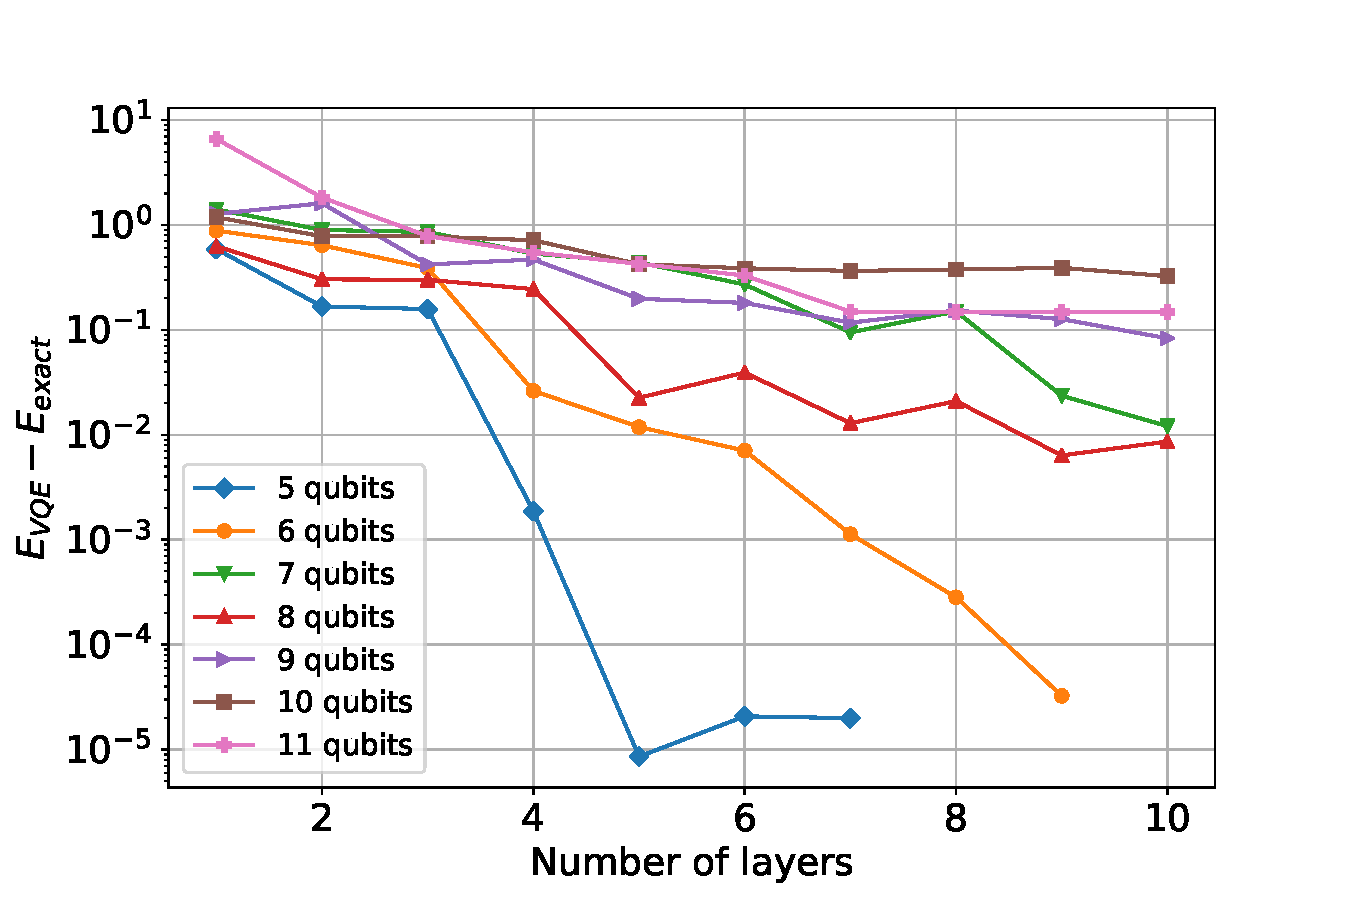
\includegraphics[width=0.7\textwidth]{figures/vqe_hubbard_nnn.pdf}
    \caption{Convergence of the VQE solution to the true ground state for the 1D next-nearest-neighbour repulsion Hubbard model versus the number of layers, on condition $V_1 = 2t, V_2 = t$. Cases of $n \leq 4$ qubits are not shown as they converged to exact solution within 2 layers. Reprinted from \cite{uvarov_variational_2020}.}
    \label{fig:vqe_hubbard_nnn}
\end{figure}

The energy error can be shown to be closely related to the infidelity between the true ground state and the variational approximation \cite{biamonte_universal_2021}. In other words, the error in energy is close to zero if the variational solution lies close to the ground state subspace. However, both of these metrics are useful only when we possess enough information on the exact solution. Since in real applications we want to find the true energy in the first place, we cannot assume this knowledge \textit{a priori}. It is therefore also interesting to consider the convergence of other physically relevant observables. Specifically, we consider the convergence of the density-density correlation function $C(m) = \langle n_0 n_m\rangle - 
\langle n_0\rangle \langle n_m\rangle$. Figure \ref{fig:correlation} shows the behavior of the density-density correlation function in the true ground state and VQE approximations.
To provide a quantitative estimate we depict relative error of the correlation function as implemented in the VQE routine with respect to the exact solution in Fig.~\ref{fig:corr_errors}. For a more serious problem, the exact solution is, of course, unavailable. Nonetheless, the convergence of the correlation function to some apparent limit can be used as an indirect sign of overall convergence. Although we did find qualitative agreement, the accuracy of the approximation, as well as the size of the spin chain, were too low to produce any reasonable quantitative estimates of the asymptotical behavior of the correlation function. 

\begin{figure}
    \centering
    \includegraphics*[width=0.7\textwidth]{figures/Correlation.pdf}
    \caption{Density-density correlation function between spatially separated lattice sites. Filled dots denote exact values as obtained by virtue of exact diagonalization of the Hamiltonian (\ref{eq:hubbard_nnn}), dashed lines denote different approximations. Here $V_1 = 2t, V_2 = t$. Reprinted from \cite{uvarov_variational_2020}.}
    \label{fig:correlation}
\end{figure}

\begin{figure}
    \centering
    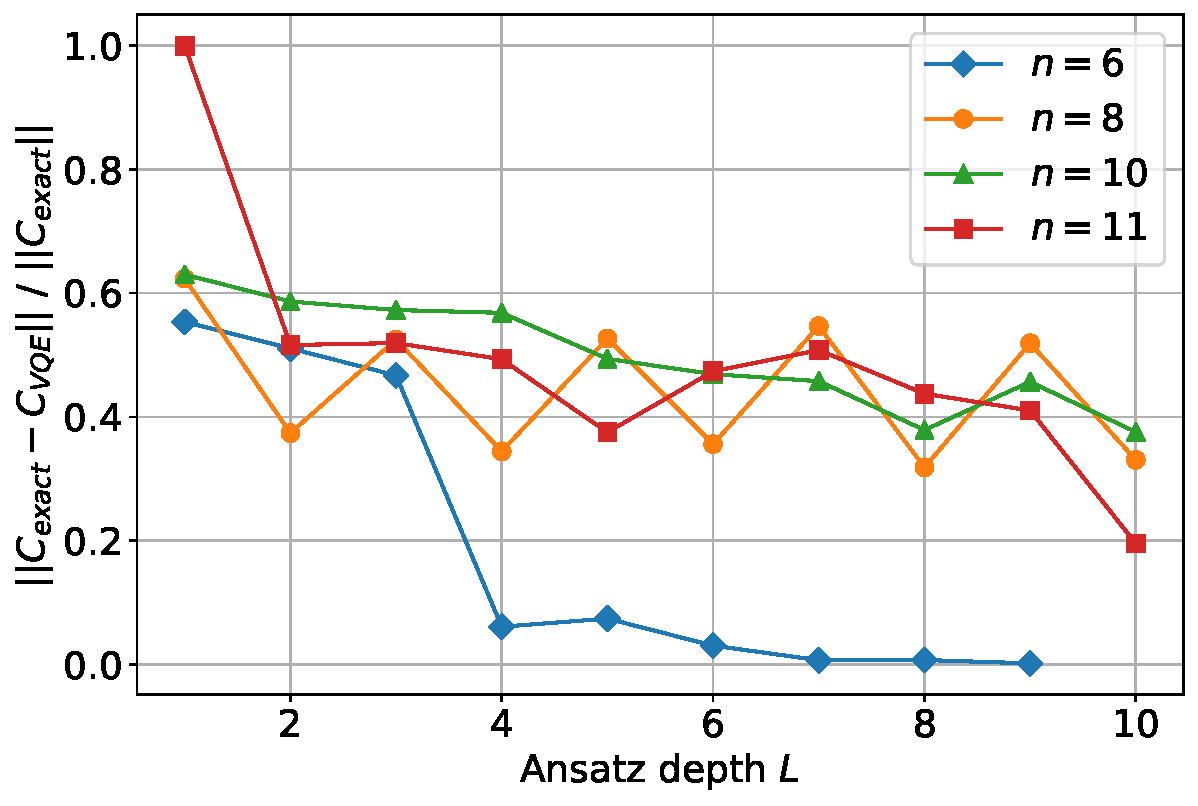
\includegraphics[width=0.7\linewidth]{figures/error_norms}
    \caption{Relative error of the correlation function as obtained with the VQE method, $C_{VQE}$, with respesect to the exact solution, $C_\mathrm{exact}$, as a function of the number of layers $L$. Reprinted from \cite{uvarov_variational_2020}.}
    \label{fig:corr_errors}
    \end{figure}{}

\subsection{Barren plateaus}

Variational algorithms can experience so-called barren plateaus \cite{mcclean_barren_2018}. While in detail this phenomenon is studied in Chapter \ref{chap:plateaus}, we will briefly explain it here as well. When we work with variational algorithms, we would like to know somehting about the optimization landscape of the problem. To do that, we can sample random points in the parameter space and consider the partial derivatives of the cost function. When the ansatz circuit is very deep, sampling unitary operators from that circuit in a certain sense very similar to sampling random unitary operators uniformly from the unitary group $U(2^n)$. Under these conditions (see Theorem \ref{thm:mcclean}), the partial derivatives $\partial_\theta \bra{\psi} H \ket{\psi}$ have zero mean and exponentially vanishing variance (in $n$).

This result, however, is valid for sufficiently long circuits with enough freedom in individual gates. Here we introduced an ansatz which preserves the number of particles in the state. A random unitary operator sampled from such an ansatz will necessarily be a direct sum of operators acting in subspaces corresponding to different particle numbers. This property is, of course, not present for random unitary operators. Another aspect of the problem is that the Hamiltonians in question also change with the number of qubits. Because of that, we performed a number of numerical experiments concerning the onset of barren plateaus in the case of Hubbard model and our ans\"atze.

Figure \ref{fig:plateaus_hubbard_ising}, top left, shows the behavior of the variance of the derivatives (averaged over random selections of $\boldsymbol{\theta}$ and $k$) for the next-nearest-neighbor Hubbard model (\ref{eq:hubbard_nnn}) under the Jordan--Wigner mapping. The particle-conserving ansatz is used for the analysis. For most qubit numbers and regardless of the model parameters, said variance drops to its limiting value even for very shallow circuits. In contrast, the same derivatives under the Bravyi--Kitaev mapping show a more gradual behavior (Figure \ref{fig:plateaus_hubbard_ising}, top right): the variance decays exponentially with the depth of the circuit. The particle-preserving gate in the ansatz was replaced with a more generic gate shown in Fig.~\ref{fig:entangler}, since the former would no longer conserve the particle number.
For comparison, we also performed a similar experiment for the transverse field Ising model. The gradient behavior away from the critical point ($h = 0.1$) and at the critical point ($h = 1$) is shown in Fig.~\ref{fig:plateaus_hubbard_ising}, bottom. In this case, the gradient variance decays exponentially with the number of layers until reaching the plateau regime for the particular number of qubits. Thus, for 4 qubits the plateau is reached right away, while for 10 qubits, 30 layers of the ansatz are still a number belonging to the transition regime. In the meantime, the criticality of the model does not seem to affect this behavior. As we will see in Chapter \ref{chap:plateaus}, a possible reason for the behavior observed in these three cases is that the Jordan--Wigner mapping produces highly nonlocal operators which are difficult to optimize.

% \todo{For BK mapping, we can plot the barren plateaus conditioned on the sample points being in the valid region (e.g.~by assuming the number of particles no more than 0.1 or 0.01 away from the correct value. We should also probably check how this depends on that number.)}

\begin{figure}
    \centering
    \begin{subfigure}{.48\linewidth}
        \centering
        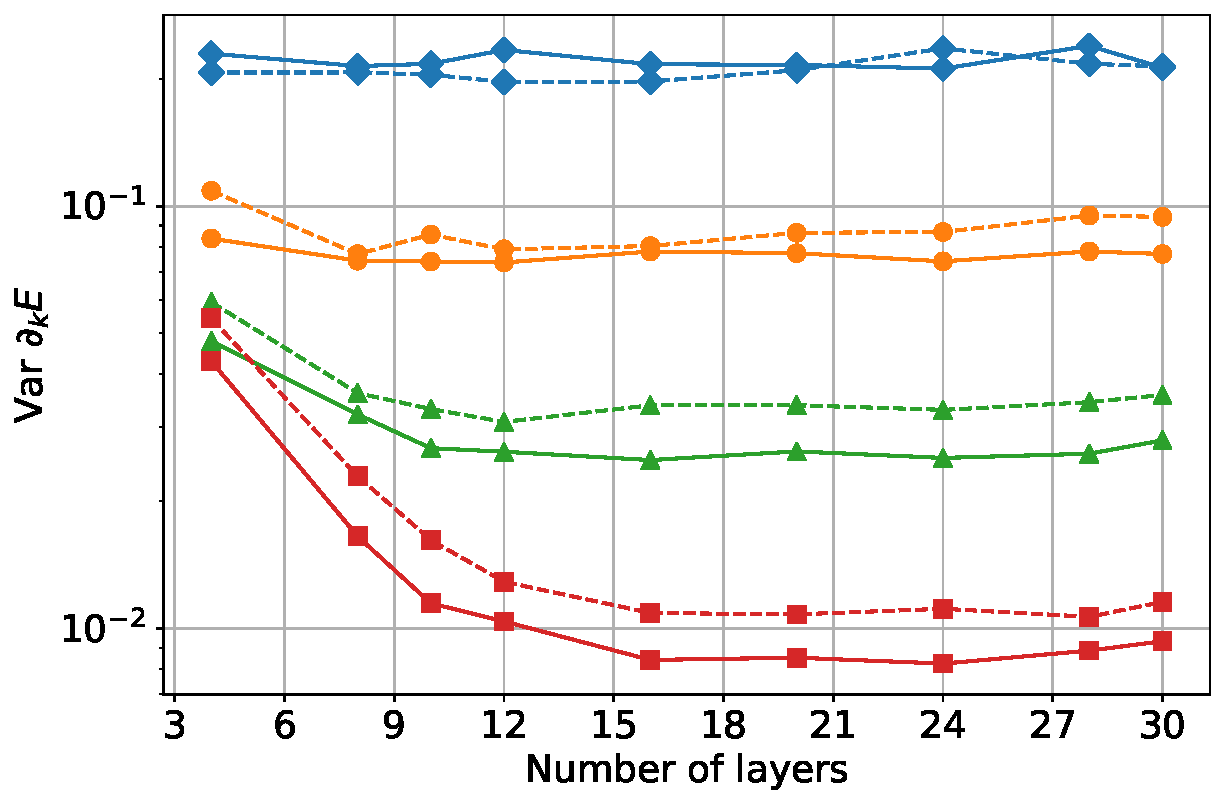
\includegraphics[width=\textwidth]{figures/plateau_hubbard_jw_both.pdf}
    \end{subfigure}\begin{subfigure}{.48\linewidth}
        \centering
        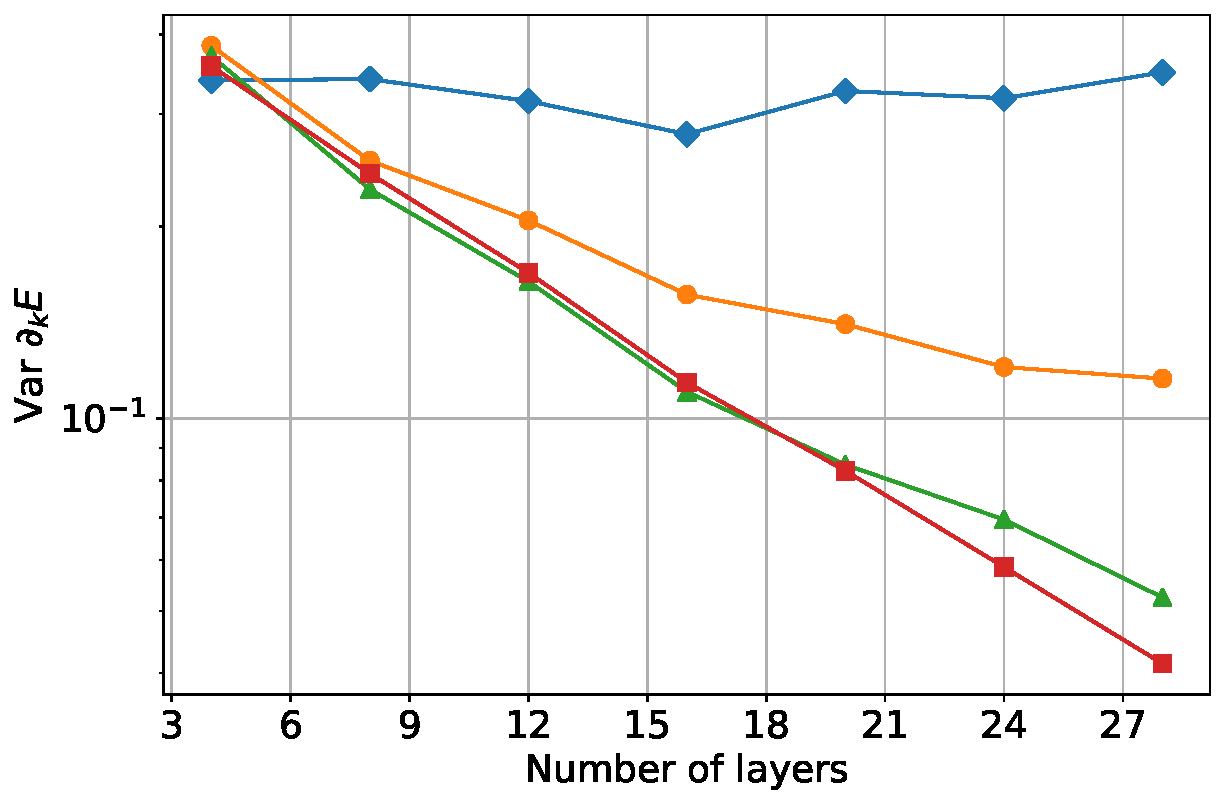
\includegraphics[width=\textwidth]{figures/plateau_hubbard_bk.pdf}
    \end{subfigure}
    \begin{subfigure}{.48\linewidth}
        \centering
        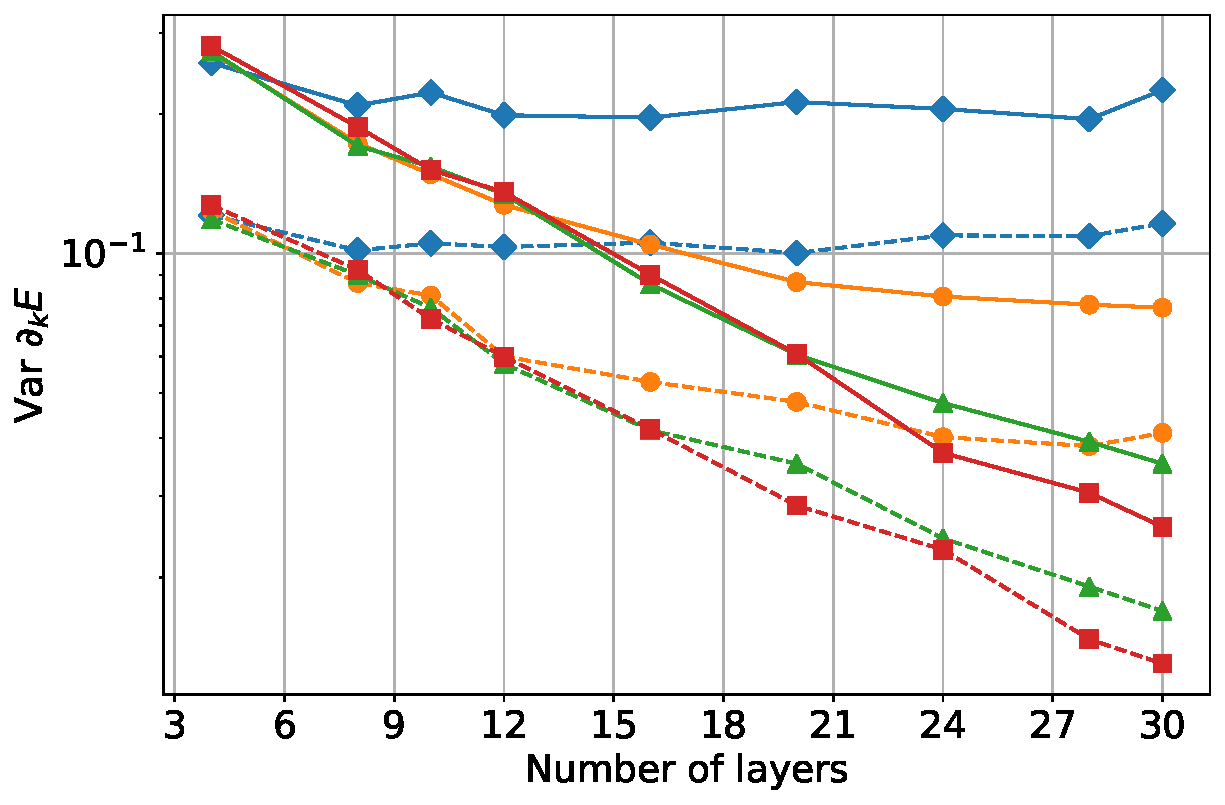
\includegraphics[width=\textwidth]{figures/plateau_ising_both.pdf}
    \end{subfigure}
    \caption{\textbf{Top left:} barren plateau effect for the Hamiltonian of Eq. (3) with
    $V_1 = t$ and $V_2 = 0$ (dashed lines), as well as $V_1 = 2t$ and $V_2 = t$
    (solid lines) versus the number of qubits as realized by virtue of
    Jordan--Wigner mapping. Diamonds: four qubits; circles: six qubits;
    triangles: eight qubits; squares: 10 qubits. \textbf{Top right:} same effect under Bravyi--Kitaev mapping, $V_1 = 2t$, $V_2 = t$.
    \textbf{Bottom:} same effect for for the transverse field Ising model of Eq. (4) away from criticality with $h = 0.1$ (dashed lines) and at the critical point $h = 1$ (solid lines).    
    Reprinted from \cite{uvarov_variational_2020}.}
    \label{fig:plateaus_hubbard_ising}
\end{figure}


\section{Discussion}

In this chapter, we saw different physical models analyzed using the VQE method. Regardless of the model, we observed a fast convergence of the energy error with the increase of the circuit depth, however, the experiments with the Hubbard model hint that this may just be the consequence of a small number of qubits, as for larger $n$ this convergence becomes less apparent.

There is a lot of choices to be made when choosing the implementation of VQE. We always have to choose the ansatz and/or its update scheme, we need to choose the optimization method, and for fermionic problems, we also have to choose the qubit encoding. A whole other set of choices not covered in this work relate to the experimental setup: how to label qubits, how many measurements to make per step, and so on. All of this affects the quality of the solution.

In the experiments with the Hubbard model we observed the barren plateau phenomenon, in which the partial derivatives converge to exponentially small values when sampled randomly. On the one hand, its behavior is to be expected: as we will see in Chapter \ref{chap:plateaus}, the locality of the operators included in the Hamiltonian is one of the key factors affecting the onset of barren plateaus. On the other hand, the theory of barren plateaus heavily relies on the concept of \textit{t-designs}, i.e.~random quantum circuits that are indistinguishable from uniformly random unitary operators under certain conditions. Clearly, the particle-conserving ansatz is not even close to resembling a uniformly random unitary, hence it is not a \textit{t}-design (again, we will back this up numerically in Chapter \ref{chap:plateaus}). Nonetheless, we observe the plateaus. This implies that in some cases the condition for observing barren plateaus is not necessarily tied to the notion of a \textit{t}-design. Alternatively, this may mean that the ansatz becomes close to a \textit{t}-design when it is restricted to the subspace with the fixed number of particles. 






